\chapter{Resultados}\label{chap:resultados}

\drop{A} continuación se va a proceder a mostrar los resultados de cada uno de los algoritmos que se han desarrollado para el sistema. Como se han realizado optimizaciones para el uso de hardware reconfigurable, al final, se realizará una comparación acerca de los tiempos de ejecución que se han obtenido.

\section{Detección de objetos}

En la figura \ref{fig:EstadosLaboratorio} se pueden observar los resultados de la aplicación del algoritmo de detección de objetos. Este algoritmo tiene dos fases. La resta de imágenes correspondiente a la figura \ref{fig:RestaObjetos} y la delimitación de objetos correspondiente a la figura \ref{fig:CuadradosObjetos}.

\begin{figure}[htbp]
 \centering
  \subfloat[Entorno con objetos]{
   \label{fig:LaboratorioObjetos}
    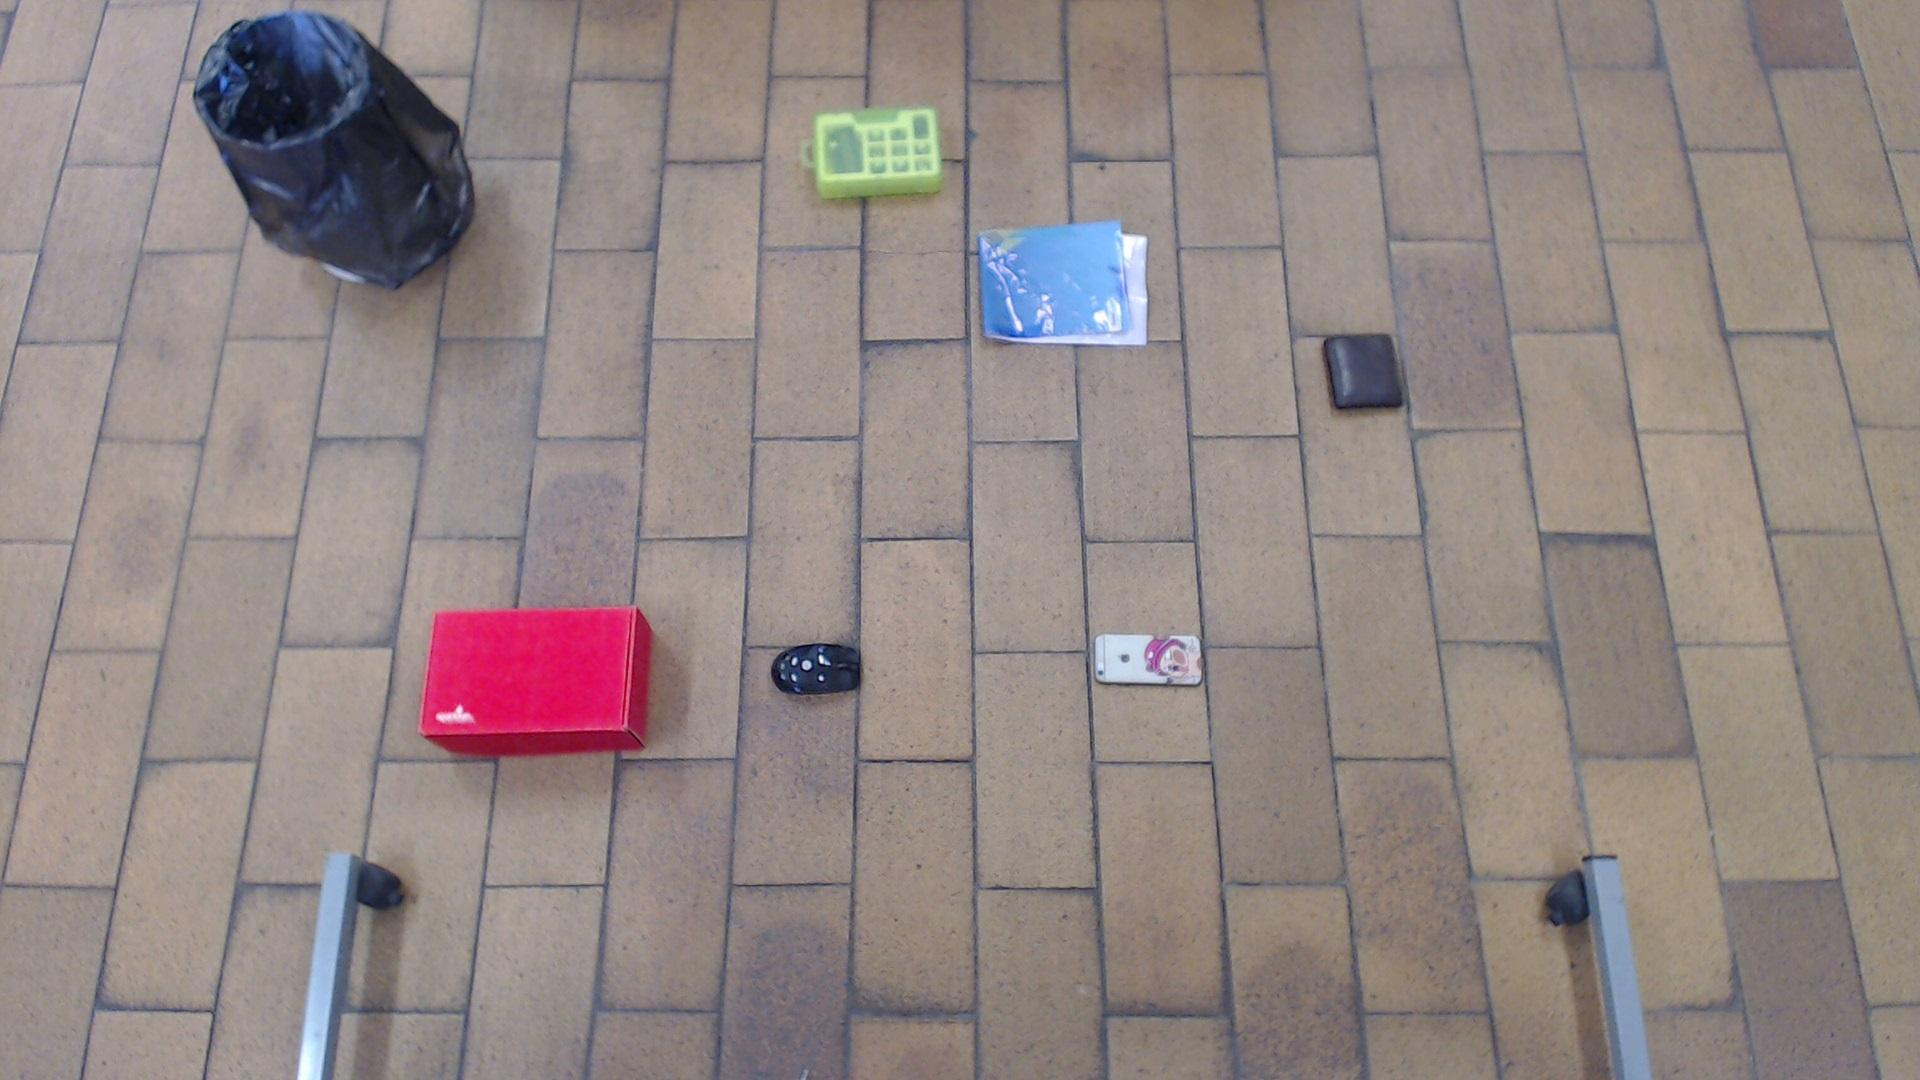
\includegraphics[width=0.33\textwidth]{./figures/LaboratorioObjetos.jpeg}}
  \subfloat[Resta de objetos]{
   \label{fig:RestaObjetos}
    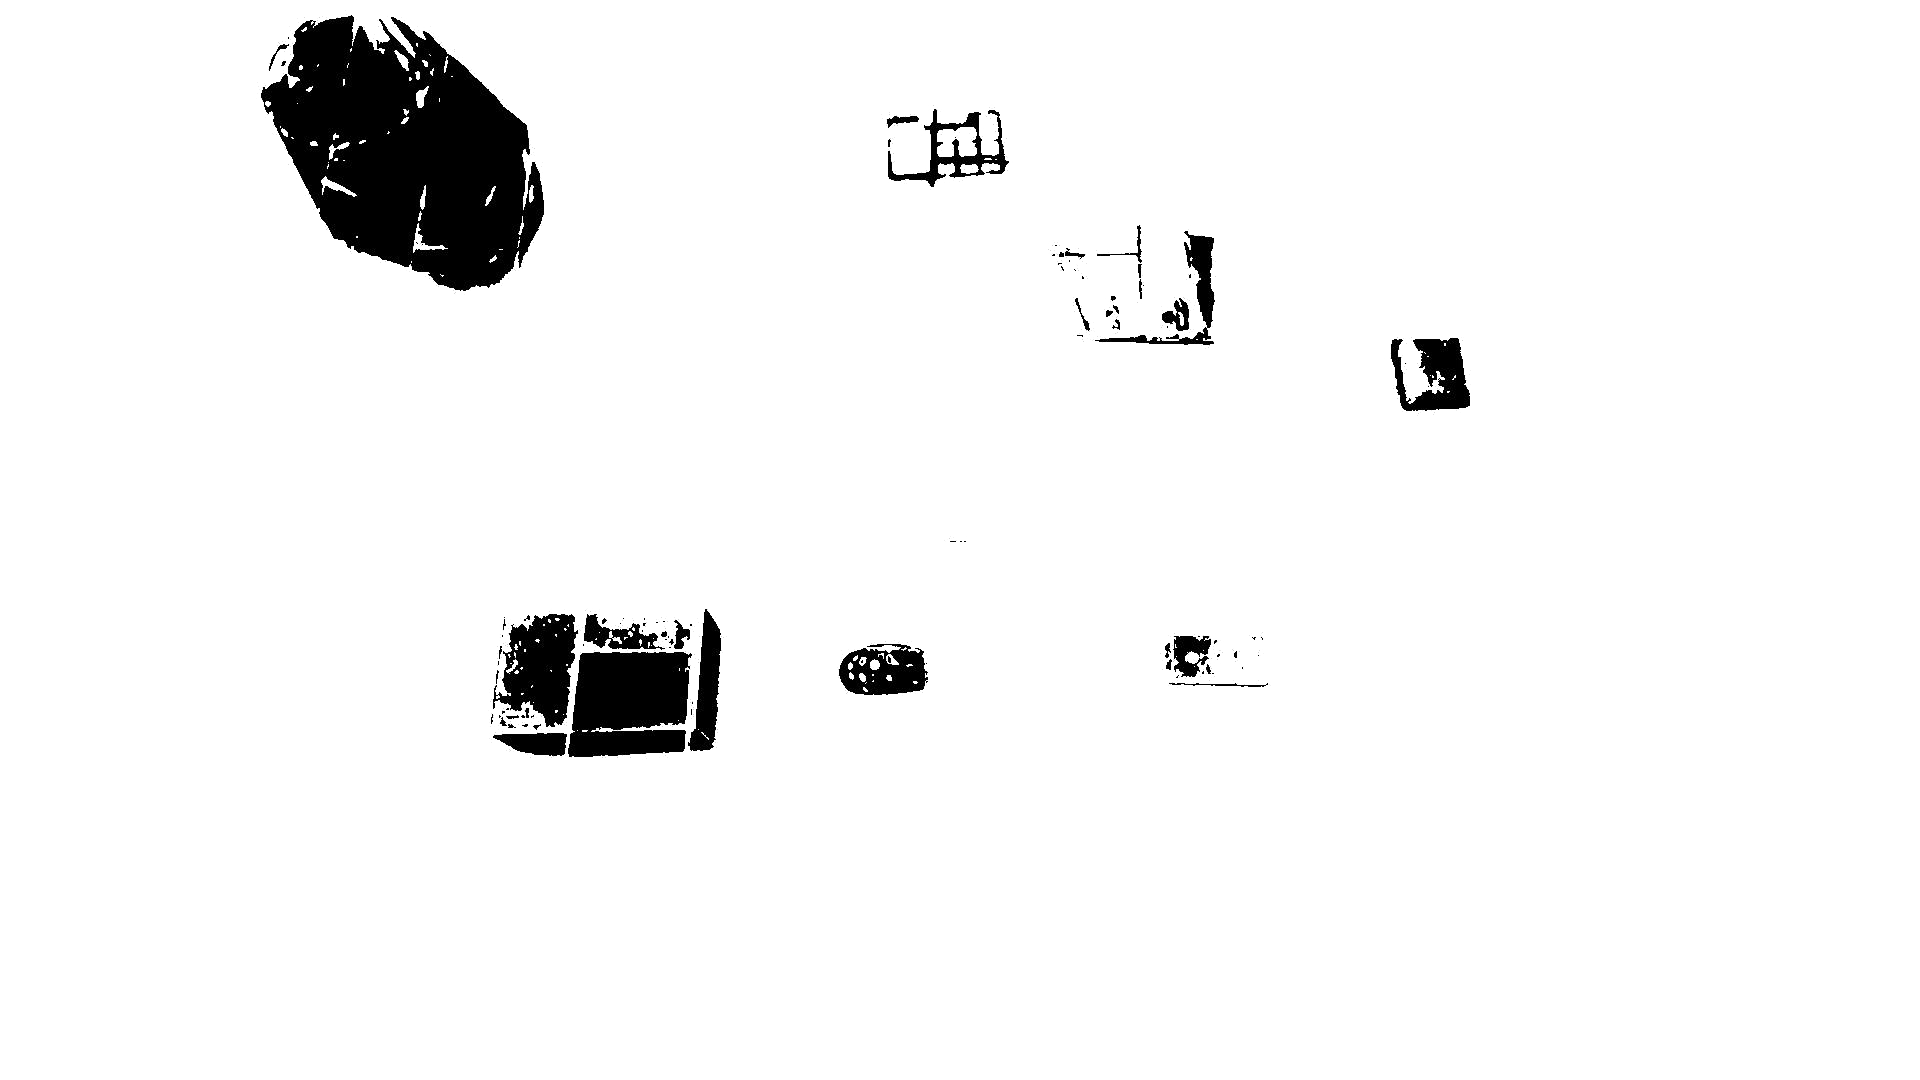
\includegraphics[width=0.33\textwidth]{./figures/RestaObjetos.jpeg}}
  \subfloat[Delimitación de obstáculos]{
   \label{fig:CuadradosObjetos}
    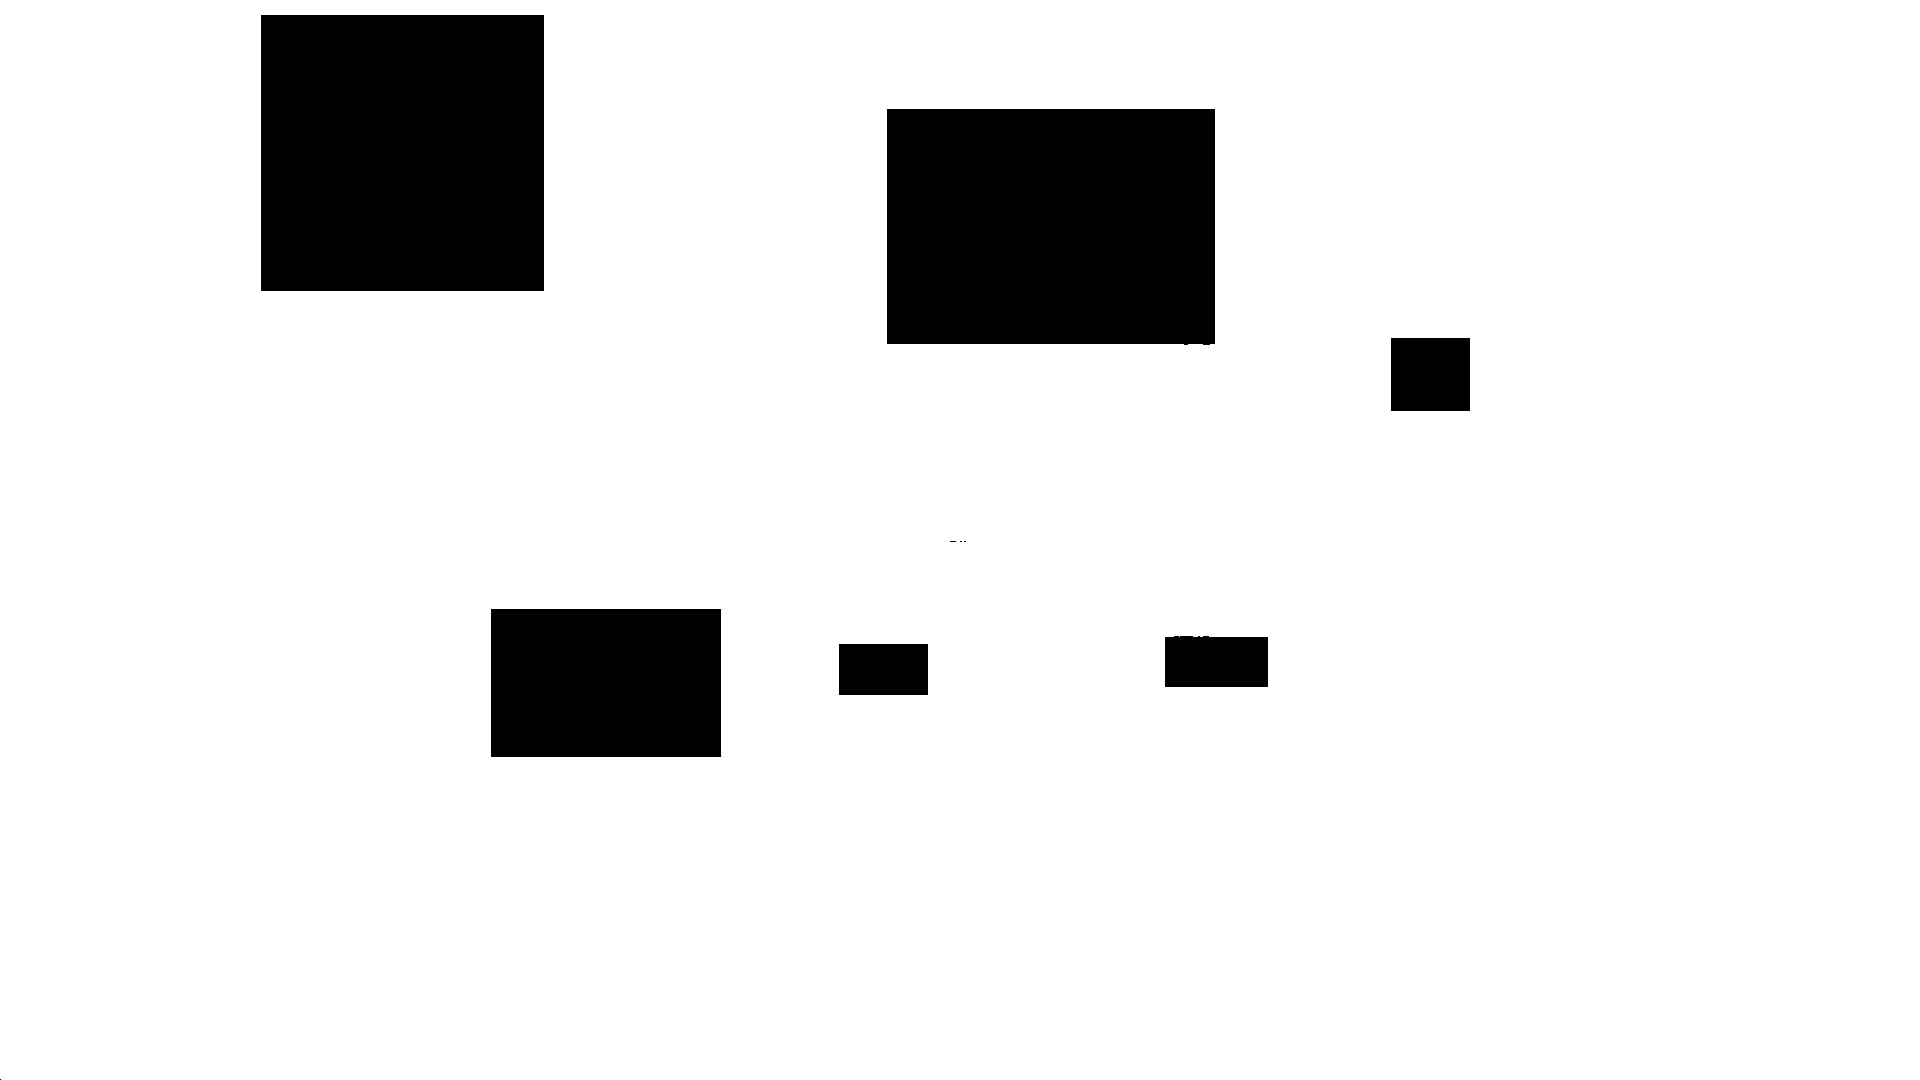
\includegraphics[width=0.33\textwidth]{./figures/CuadradosObjetos.jpeg}}
 \caption{Ejemplo de aplicación del algoritmo de detección de objetos}
 \label{fig:EstadosLaboratorio}
\end{figure}



\section{Detección del vehículo frente a los objetos}

En la figura \ref{fig:deteccionVehiculo1} se puede observar como funciona el algoritmo de detección del vehículo frente a los objetos. El círculo verde que aparece sobre el coche ha sido incluido por el algoritmo. La imagen original es exactamente igual salvo con el círculo verde. En la imagen de la izquierda se puede observar un círculo blanco sobre la imagen que corresponde a la posición del vehículo. Se calcula el punto medio del círculo y se genera el fichero correspondiente que guarda las coordenadas.

\begin{figure}[htbp]
 \centering
    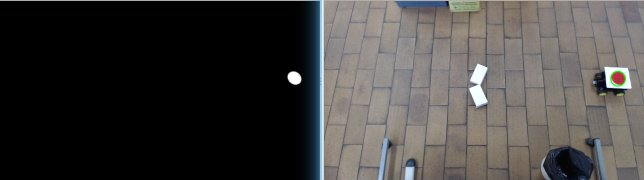
\includegraphics[width=.95\textwidth]{./figures/deteccionvehiculo2.jpeg}
 \caption{Ejemplo de detección de la posición del vehículo en el entorno.}
 \label{fig:deteccionVehiculo1}
\end{figure}

\section{Modificación algoritmo A* \cite{ImplementacionAlgoritmoA}}

En la figura \ref{fig:ResultadoAEstrella} se puede observar el cálculo de la trayectoria para el escenario con objetos \ref{fig:objetos}. La línea de color verde corresponde a la ruta.

\begin{figure}[htbp]
 \centering
  \subfloat[Resta de objetos]{
   \label{fig:objetos}
    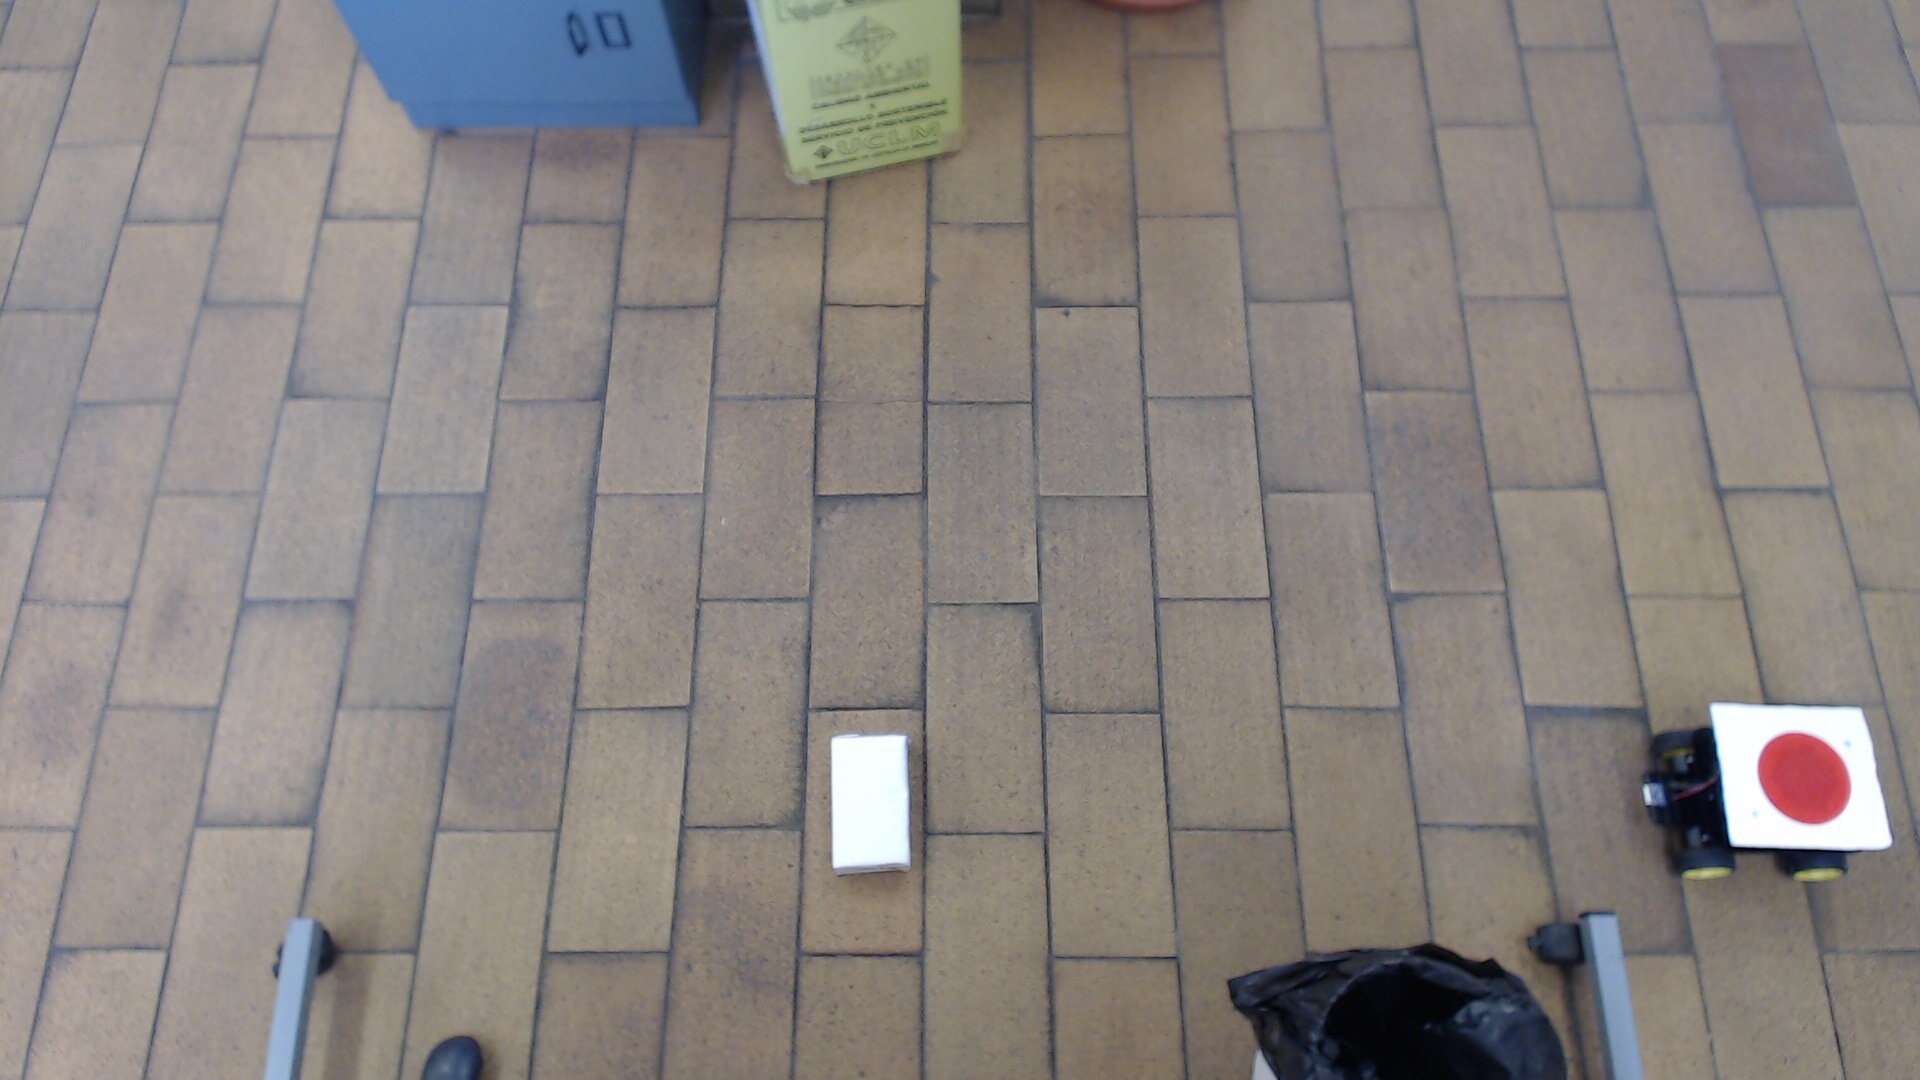
\includegraphics[width=0.475\textwidth]{./figures/scenarioCoordinador.jpg}}
  \subfloat[Escenario de pruebas]{
   \label{fig:ruta}
    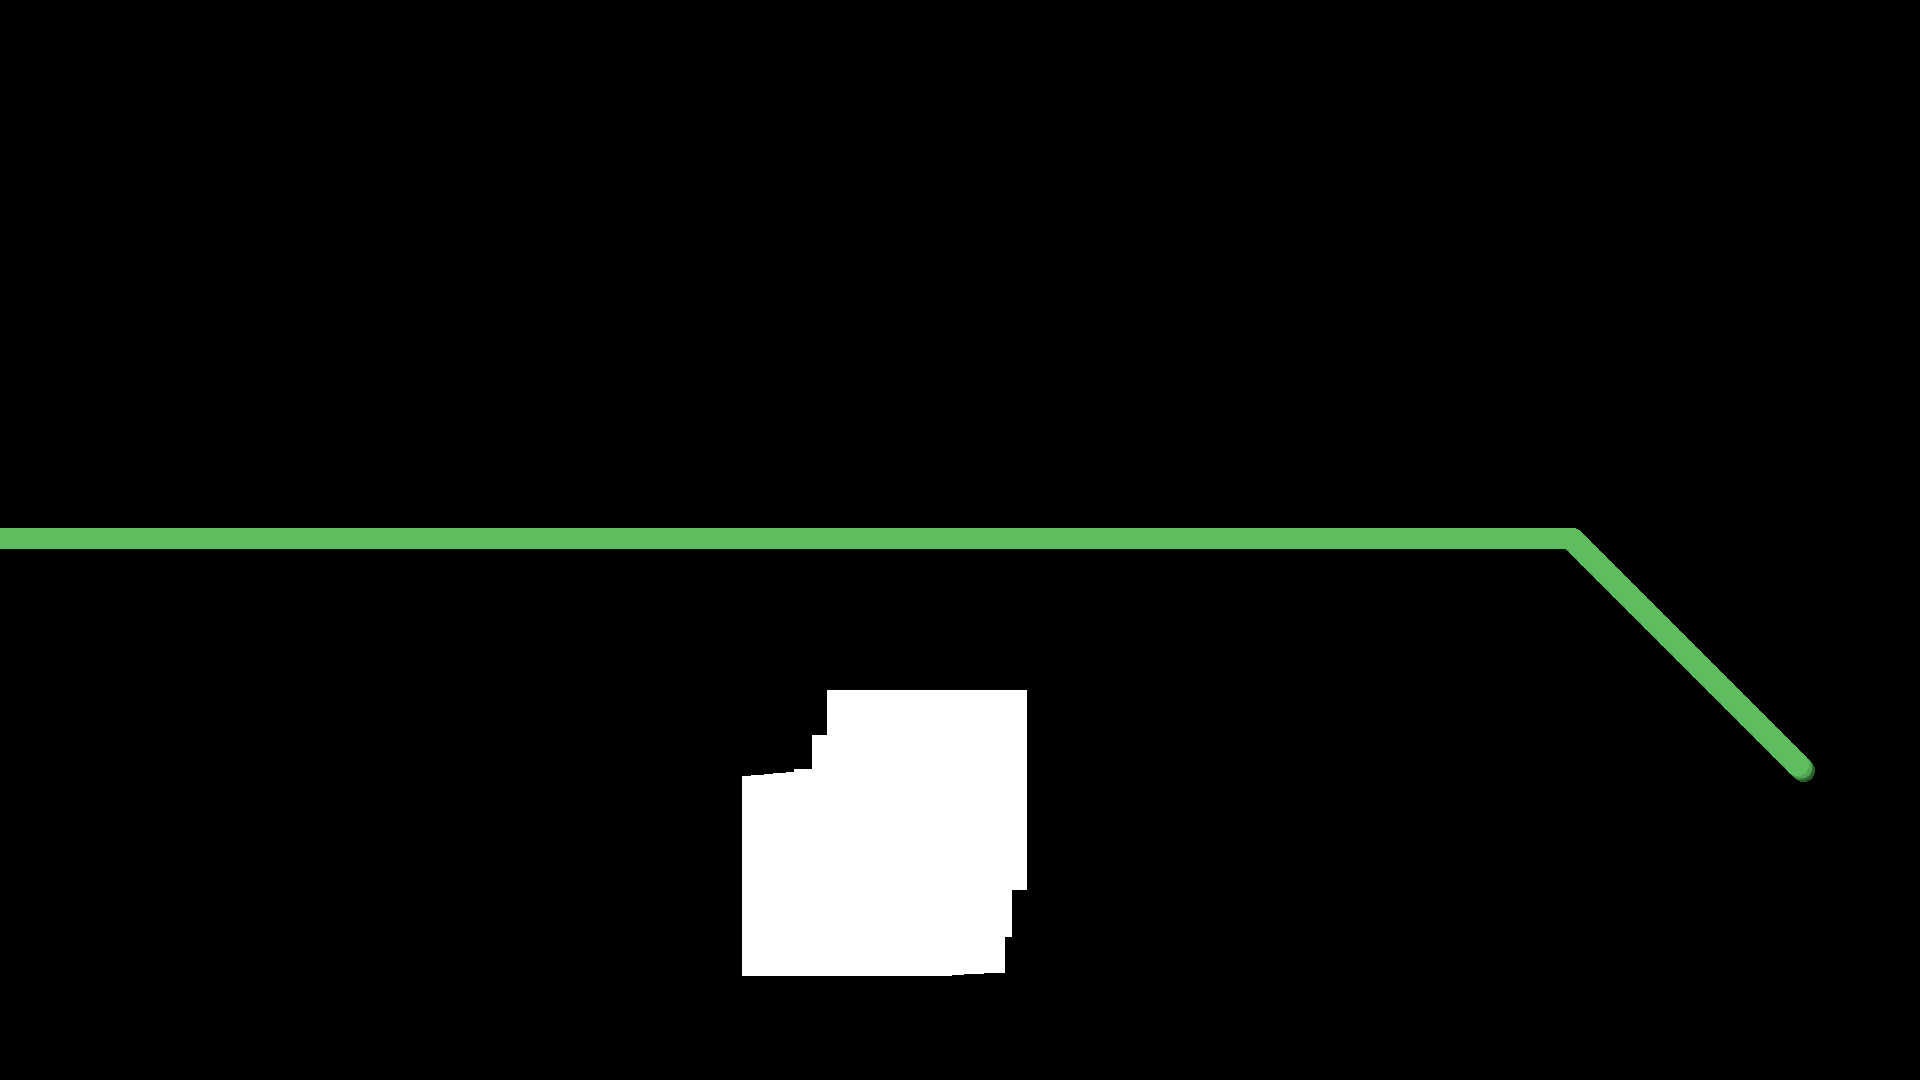
\includegraphics[width=0.475\textwidth]{./figures/pathCoordinador.jpeg}}
 \caption{Ejemplo de cálculo de trayectoria}
 \label{fig:ResultadoAEstrella}
\end{figure}

\section{Comunicación}

La comunicación por el puerto serie tiene como resultado los cuatro casos distintos que aparecen en la figura \ref{fig:ComunicacionRes}.

\begin{figure}[htbp]
 \centering
  \subfloat[Esperando movimiento]{
   \label{fig:scenarioCoordinador}
    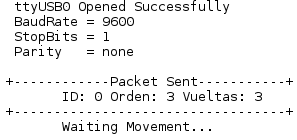
\includegraphics[width=0.25\textwidth]{./figures/capturaComunicacion1.png}}
  \subfloat[Movimiento realizado]{
   \label{fig:pathCoordinador}
    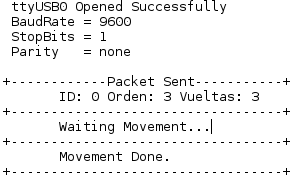
\includegraphics[width=0.25\textwidth]{./figures/capturaComunicacion3.png}}
  \subfloat[Timeout]{
   \label{fig:ruta}
    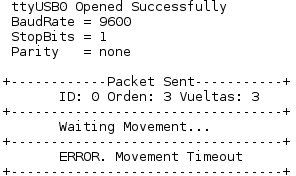
\includegraphics[width=0.25\textwidth]{./figures/capturaComunicacion2.png}}
  \subfloat[Paquete erróneo]{
   \label{fig:ruta}
    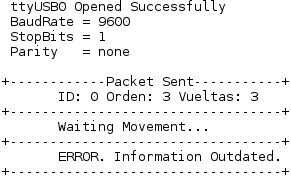
\includegraphics[width=0.25\textwidth]{./figures/capturaComunicacion4.png}}
 \caption{Comunicación por el puerto serie}
 \label{fig:ComunicacionRes}
\end{figure}

\section{Coordinador de los movimientos del vehículo}

Para los resultados del coordinador de los movimientos del vehículo se ha decidido mostrar la figura \ref{fig:Coordinador} que corresponde a la trayectoria que debe seguir el vehículo y una captura de pantalla de los paquetes que han sido enviados por el puerto serie para realizar el movimiento.

\begin{figure}[htbp]
 \centering
  \subfloat[Escenario de pruebas]{
   \label{fig:scenarioCoordinador}
    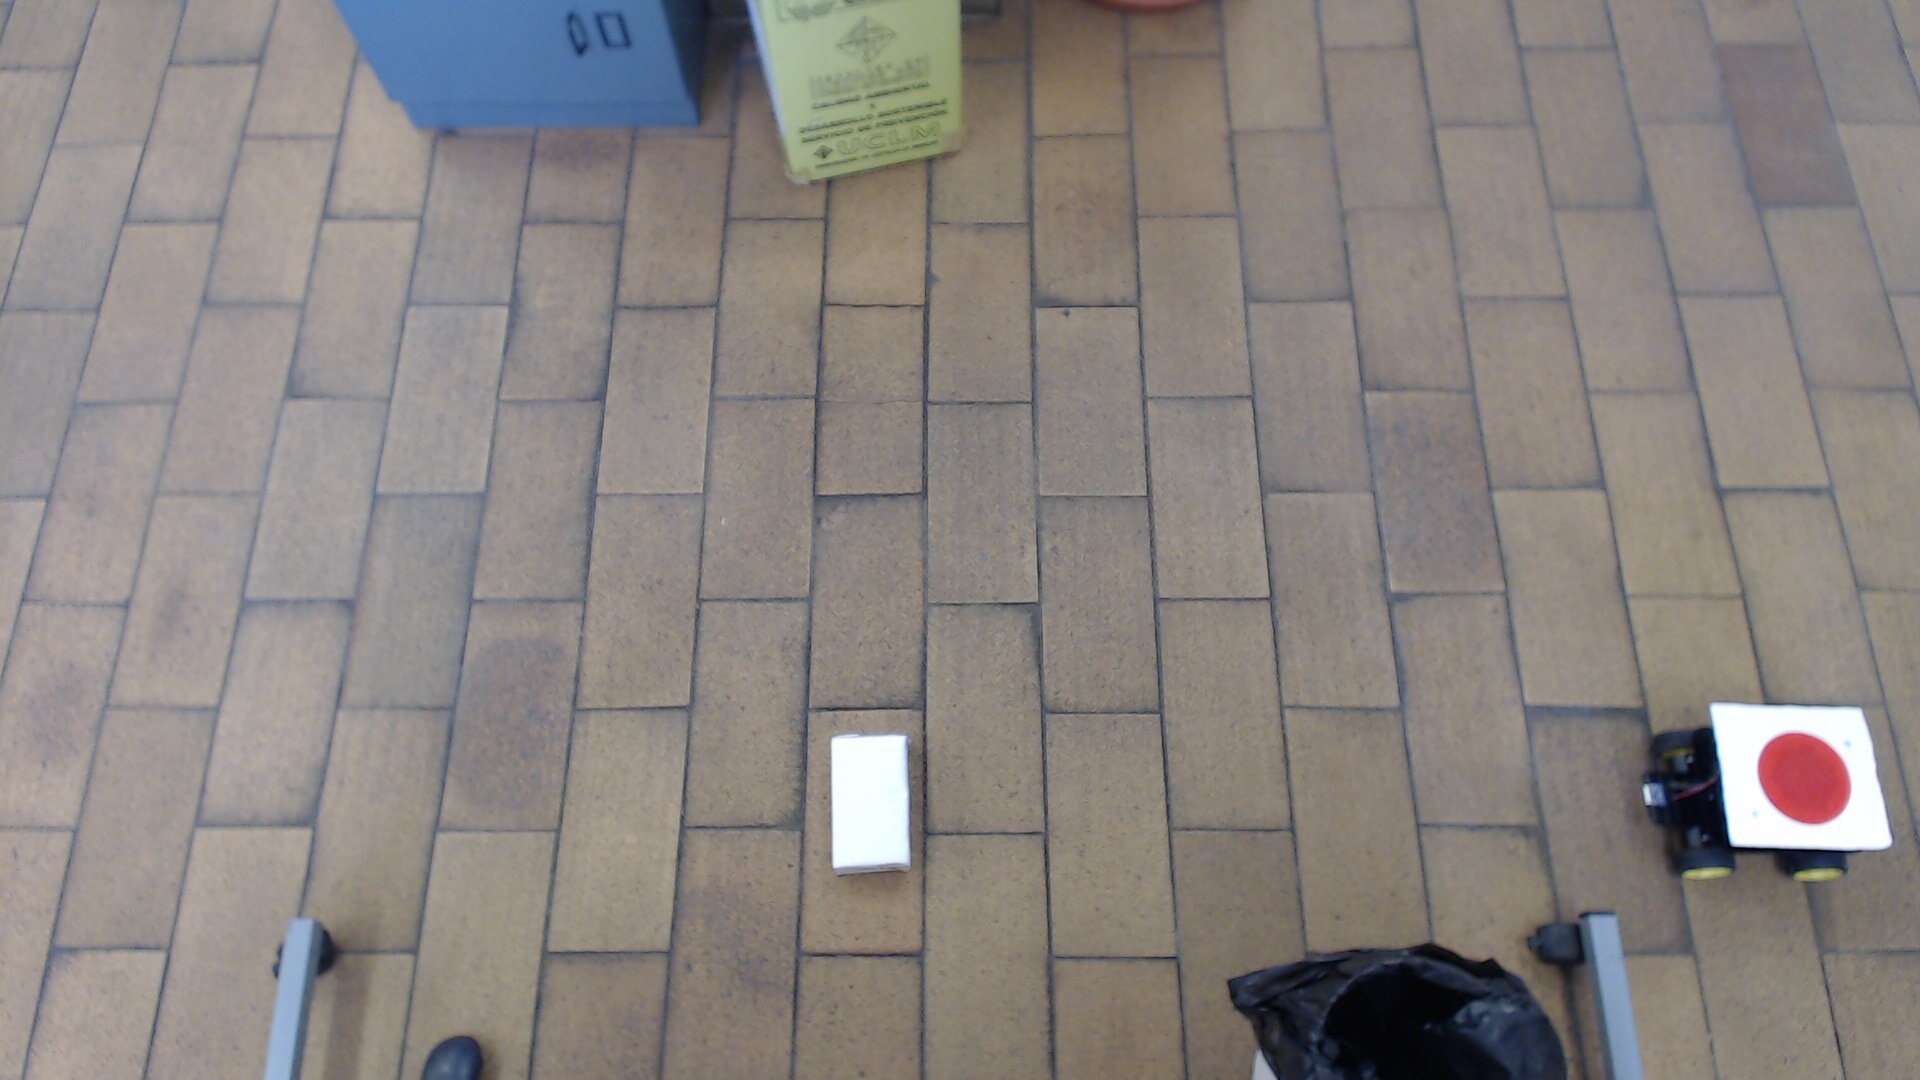
\includegraphics[width=0.33\textwidth]{./figures/scenarioCoordinador.jpg}}
  \subfloat[Ruta calculada]{
   \label{fig:pathCoordinador}
    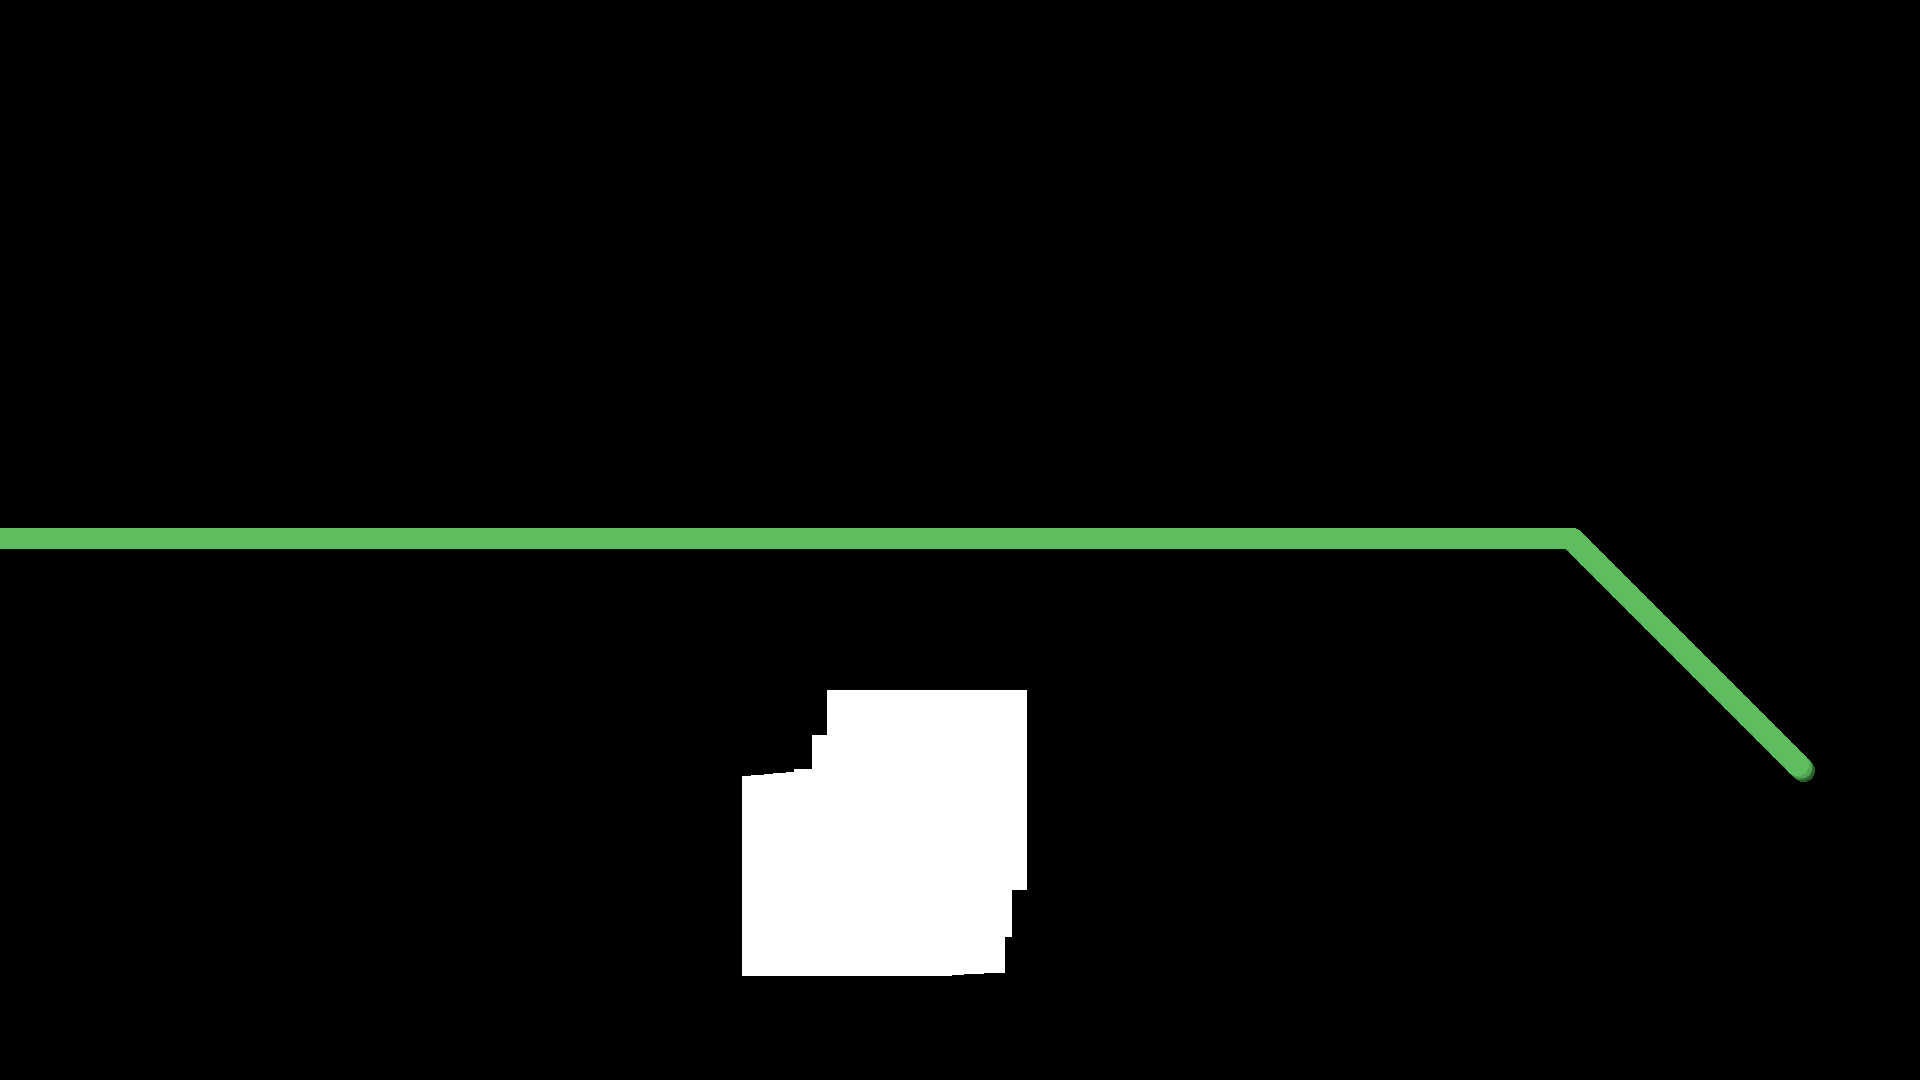
\includegraphics[width=0.33\textwidth]{./figures/pathCoordinador.jpeg}}
  \subfloat[Paquetes enviados]{
   \label{fig:ruta}
    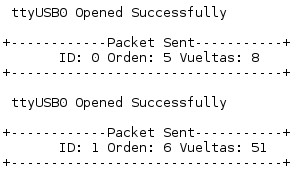
\includegraphics[width=0.33\textwidth]{./figures/capturaCoordinador.png}}
 \caption{Ejemplo de envío de movimientos al vehículo}
 \label{fig:Coordinador}
\end{figure}

\section{Integración del sistema}

A continuación se han expuesto en el cuadro \ref{tab:TiempoEjecucionSistemaMalo} los tiempos de ejecución del sistema para el escenario de la figura \ref{fig:EscenarioPruebaFinal}. Como se puede observar el cuello de botella de nuestra aplicación es el algoritmo de cálculo de trayectoria, el cual puede llegar a limitarnos, en algunas circunstancias, la ejecución en tiempo real debido a sus largos tiempos de cálculo. Por ello, se ha decidido realizar una serie de optimizaciones en el sistema para mejorar los tiempos de ejecución y la versatilidad en cuanto a los formatos de imagen que se utilizan como argumentos.

\begin{figure}[htbp]
 \centering
  \subfloat[Escenario sin objetos]{
   \label{fig:scenarioCoordinador}
    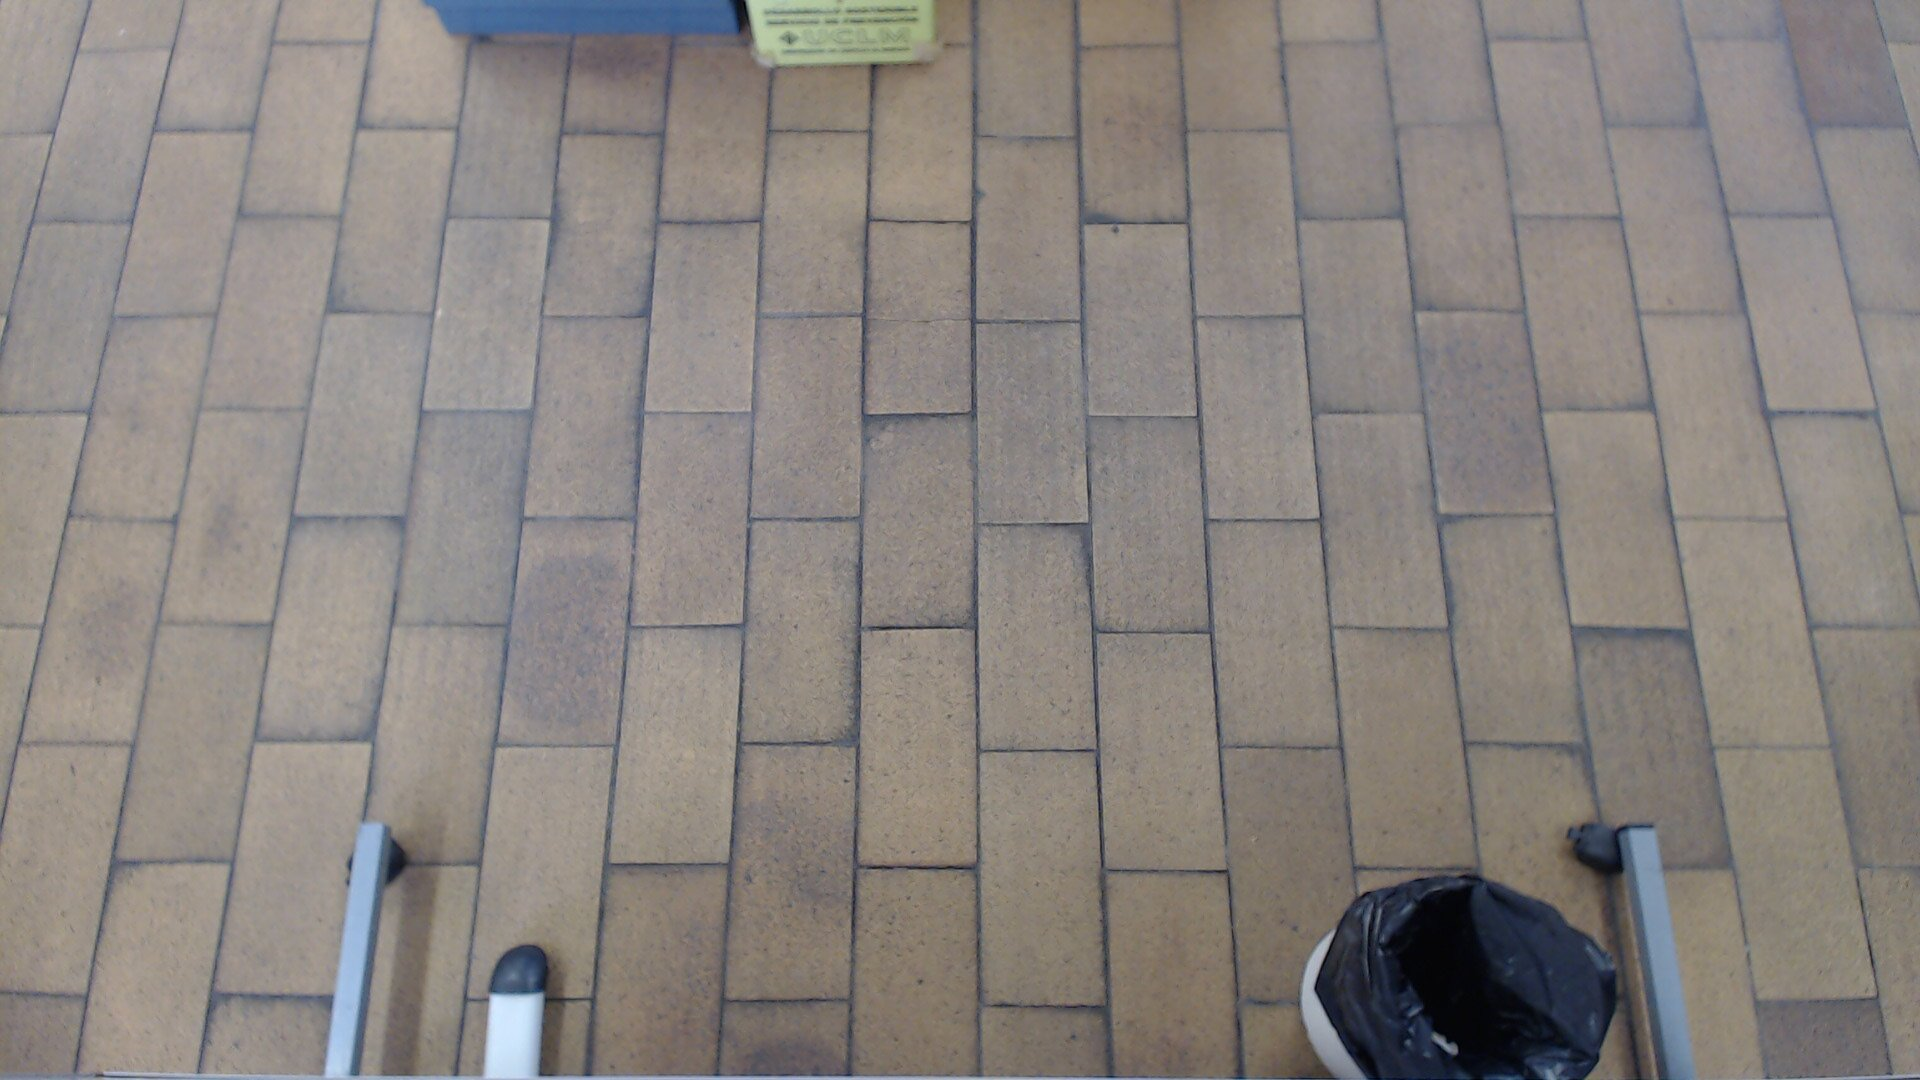
\includegraphics[width=0.33\textwidth]{./figures/scenarioFinal.jpg}}
  \subfloat[Escenario con objetos]{
   \label{fig:pathCoordinador}
    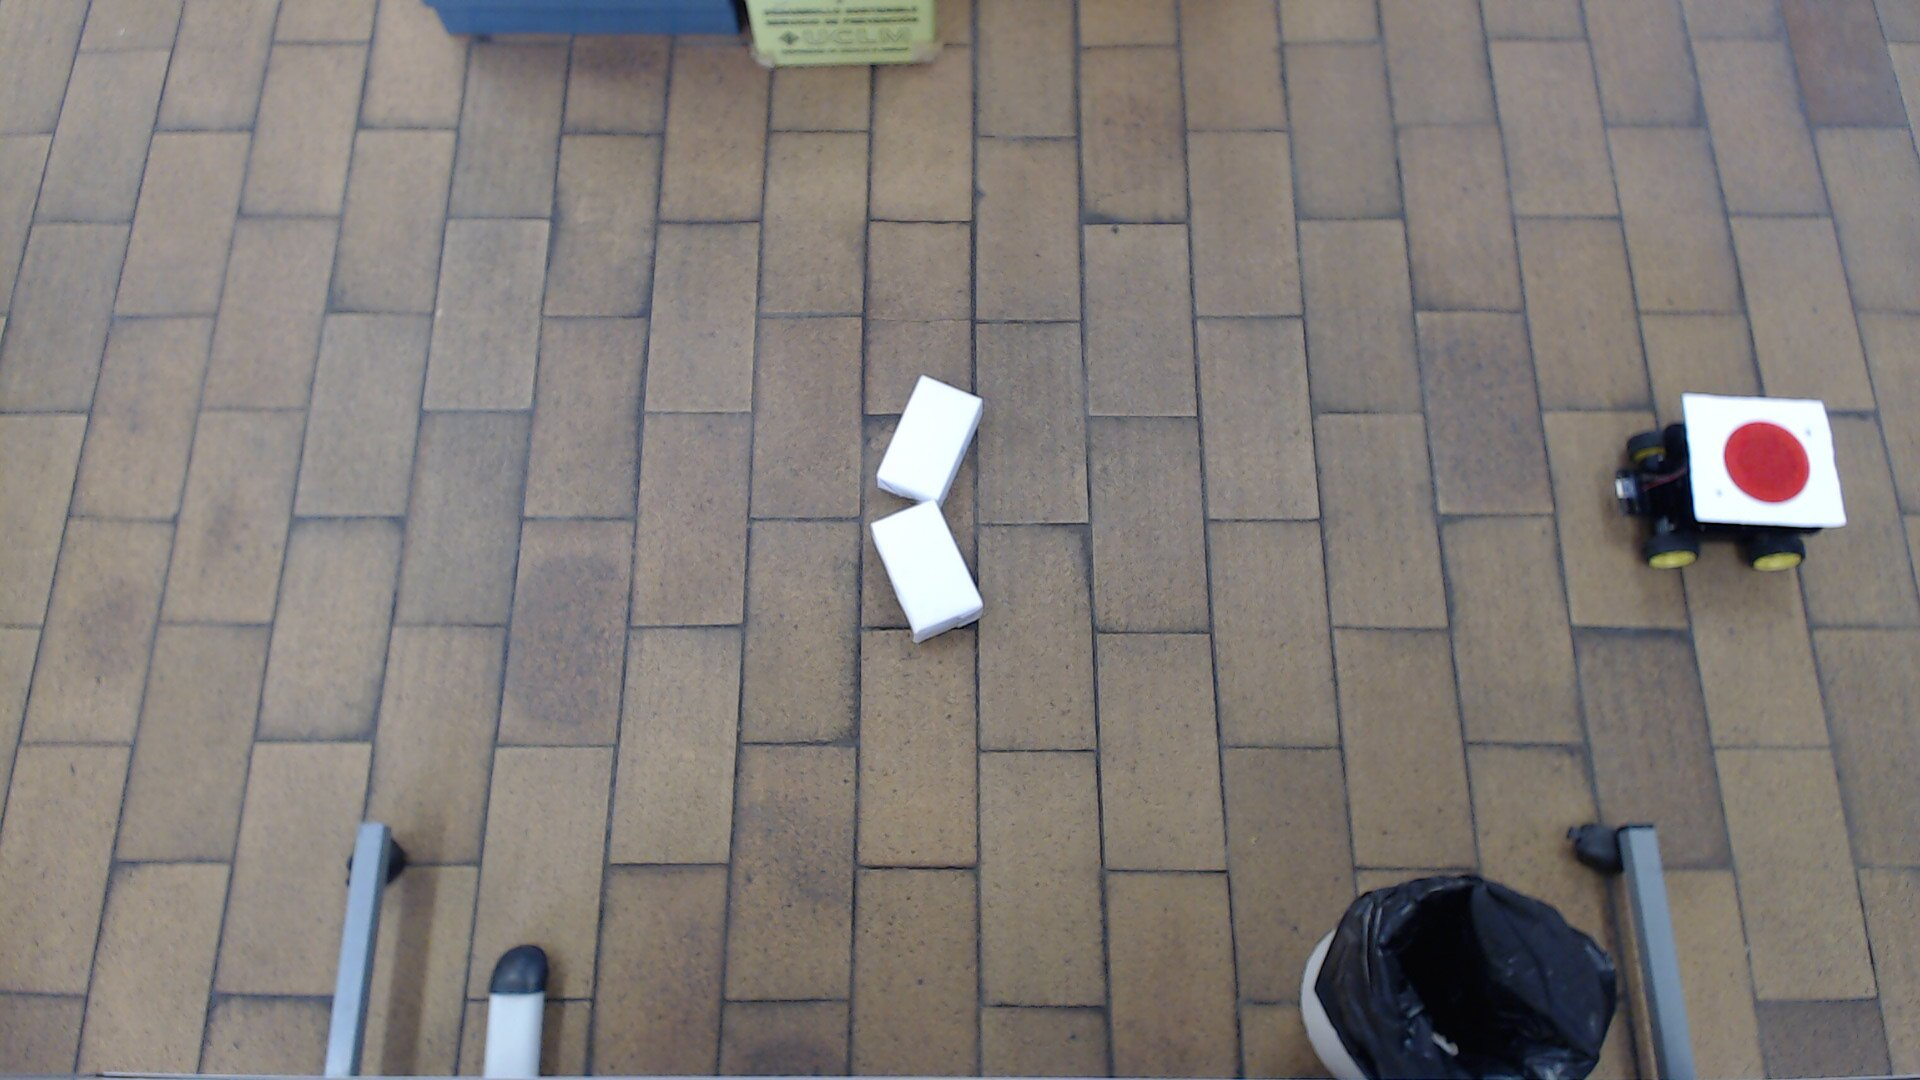
\includegraphics[width=0.33\textwidth]{./figures/scenarioVehicleFinal.jpg}}
  \subfloat[Ruta calculada]{
   \label{fig:rutafinal}
    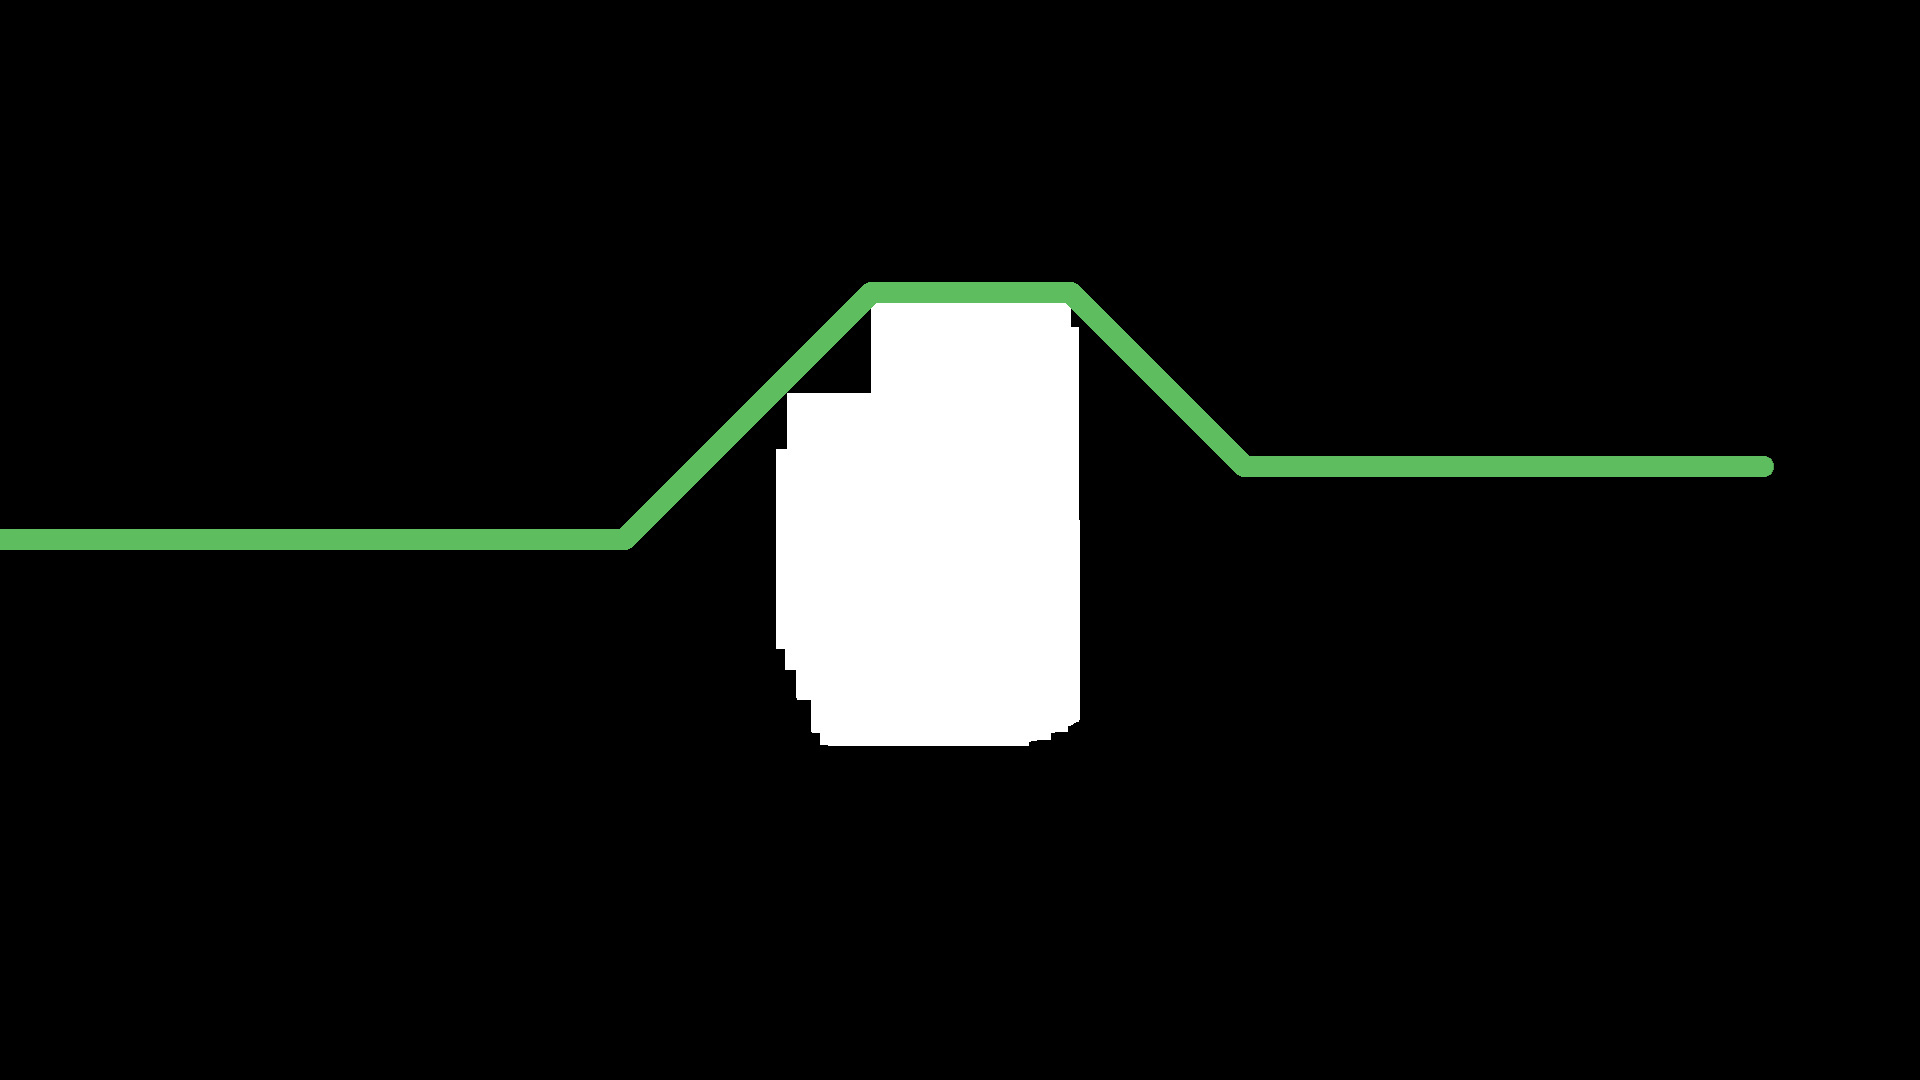
\includegraphics[width=0.33\textwidth]{./figures/rutaFinal.jpeg}}
 \caption{Escenario con el que se ha realizado la medición de los tiempos}
 \label{fig:EscenarioPruebaFinal}
\end{figure}


\begin{table}[hbtp]
\centering
\begin{tabular}{|l|l|}
\hline
\multicolumn{2}{|c|}{\cellcolor[HTML]{9B9B9B}Tiempos de ejecución del sistema} \\ \hline
Detección vehículo                           & 0.30 seg                      \\ \hline
Detección objetos                            & 0.50 seg                      \\ \hline
Cálculo de trayectoria                       & 7.66 \textbf{min}             \\ \hline
\end{tabular}
\caption {Tiempos de ejecución del sistema sin optimizar}
\label{tab:TiempoEjecucionSistemaMalo}
\end{table}
 

\section{Optimizaciones realizadas}

Se va a proceder a enumerar los resultados obtenidos tras la aplicación de las optimizaciones realizadas en el sistema. En el cuadro \ref{tab:TiempoEjecucionSistemaOptimizado} se muestran los tiempos de ejecución del sistema optimizado para el caso de estudio de la figura \ref{fig:EscenarioPruebaFinal}.

\begin{table}[hbtp]
\centering
\begin{tabular}{|l|l|}
\hline
\multicolumn{2}{|c|}{\cellcolor[HTML]{9B9B9B}Tiempos de ejecución del sistema} \\ \hline
Detección vehículo                           & 0.30 seg                      \\ \hline
Detección objetos                            & 0.41 seg                      \\ \hline
Cálculo de trayectoria                       & 0.0030 seg                     \\ \hline
\end{tabular}
\caption {Tiempos de ejecución del sistema optimizado}
\label{tab:TiempoEjecucionSistemaOptimizado}
\end{table}
 

\subsection{Tratamiento de imágenes en varios formatos}

Originalmente el sistema estaba diseñado para utilizar imágenes en formato \ac{BMP}, pero mediante la utilización de la librería \emph{OpenCV} se ha logrado ampliar el número de formatos permitidos a \ac{BMP}, \ac{JPEG}, \ac{TIFF} y \ac{PNG} entre otros. Actualmente se utilizan imágenes en formato \ac{JPG} debido a que el tamaño de las imágenes varía de 3,7 \ac{MB} por imagen \emph{FullHD} a color en formato \ac{BMP} a unos 300 \acs{KB} por imagen \emph{FullHD} a color en formato \ac{JPG}. Además, el uso de la función \emph{imread} genera una matriz tipo \emph{Mat} que permite interactuar con muchos tipos de funciones para tratamiento de imágenes. 

\subsection{Detección de obstáculos con \emph{OpenCV}}

Tras haber desarrollado el algoritmo de delimitación de obstáculos se realizaron una serie de pruebas y se comprobó que en algunos casos no daba los resultados esperados. Es por ello, que se buscó una solución más fiable a la delimitación de objetos mediante el uso de la librería \emph{OpenCV}. Se decidió utilizar la función \emph{dilate} ya que nos permite ampliar los objetos detectados en función de un tamaño como parámetro.

\subsection{Segmentación de la imagen en macrobloques}

Ya que el algoritmo de cálculo de trayectoria es la limitación principal en cuanto a la posibilidad de ejecutar el sistema en tiempo real se decidió buscar una optimización para mejorar el tiempo de ejecución del algoritmo. Para realizar una comparación entre algoritmos veasé los cuadros \ref{tab:TiempoEjecucionSistemaMalo} y \ref{tab:TiempoEjecucionSistemaOptimizado}.

\subsection{A* optimizado para \emph{Vivado} \acs{HLS}}

Debido a que el algoritmo de cálculo de trayectoria es el cuello de botella del sistema, se decidió embeber el algoritmo en hardware reconfigurable para mejorar el tiempo de ejecución. Para ello ha sido necesario realizar una nueva implementación del algoritmo que cumpla las restricciones de la herramienta \emph{Vivado} \ac{HLS}. Una vez lograda la implementación, se realizó la síntesis del algoritmo y estos son los datos más relevantes que nos ha mostrado la herramienta.

\section{Integración del sistema en la placa \emph{Zedboard}}

Para esta sección se van a mostrar las estadísticas que ha generado la síntesis del algoritmo A* en la herramienta \emph{Vivado} \ac{HLS}.

Como se puede observar en la figura \ref{fig:periodoEstimado} el tiempo ciclos de reloj estimado es de 8,48 ns. Gracias a que la suma entre el tiempo estimado e incertidumbre es menor que el objetivo se puede puede llevar a cabo el uso de una frecuencia de 100 \acs{MHz}.

\begin{figure}[htbp]
 \centering
    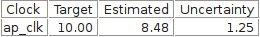
\includegraphics[width=.6\textwidth]{./figures/PeriodoEstimado.jpeg}
 \caption{Periodo de reloj estimado para el algoritmo A*}
 \label{fig:periodoEstimado}
\end{figure}

A continuación se puede observar en la figura \ref{fig:loop} el número de iteraciones por bucle que contiene el algoritmo A*. El bucle 4 y 5 son indeterminados debido a que la condición de de finalización no es determinista. Ya que están relacionadas con la resolución del cálculo de la ruta.

\begin{figure}[htbp]
 \centering
    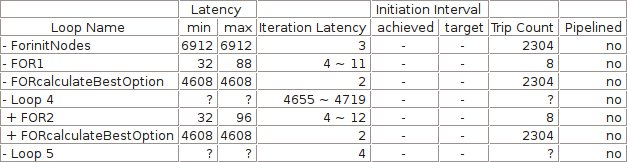
\includegraphics[width=1\textwidth]{./figures/loop.jpeg}
 \caption{Latencias para cada bucle del algoritmo A*}
 \label{fig:loop}
\end{figure}

Por último se van a mostrar los recursos necesarios para la ejecución del algoritmo en la placa \emph{Zedboard}, véase la figura \ref{fig:recursos}.

\begin{figure}[htbp]
 \centering
    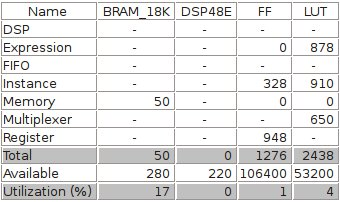
\includegraphics[width=.7\textwidth]{./figures/recursos.jpeg}
 \caption{Recursos necesarios para la ejecución del algoritmo A*}
 \label{fig:recursos}
\end{figure}

